% Import Packages
\documentclass[12pt,a4paper]{article}
\usepackage[utf8]{inputenc}
\usepackage{amsmath,amsfonts,amssymb} %math related
\usepackage{fancyhdr} %fancy headers
\pagestyle{fancy} %something to do with page layout
\usepackage{float} %control over positions of figures etc
\usepackage{graphicx} %importing graphics
\usepackage{hyperref} %refrencing
\usepackage{relsize} %text changing sizes
\usepackage{tabularx} %table controls
%\usepackage{times} %times new roman font
\usepackage{titling} %fancy titles
\newcommand{\textsub}{\textsubscript}
% make command for \subtitle
\newcommand{\subtitle}[1]{%
  \posttitle{%
    \par\end{center}
    \begin{center}\large#1\end{center}
    \vskip0.4em}%
}


%Title Page
\title{WTFpga?}
\author{{Developed by Joe FitzPatrick} \\
		{FOSSified by Piotr Esden-Tempski and Clifford Wolf}\\
		{Presented by Josh Johnson}} 


%set margins
\usepackage[left=2.5cm,right=2.5cm,top=2.5cm,bottom=2.5cm,headheight=1cm]{geometry}
\fancyheadoffset{0cm}
\lhead{WTFpga?}
\chead{}
\rhead{}
\lfoot{}
\cfoot{}
\rfoot{\thepage}
\renewcommand{\headrulewidth}{0.4pt}

\begin{document}
%Title Page
\begin{titlingpage}
    \maketitle
\end{titlingpage}

\newpage

\section{Introduction}
Welcome to the workshop! This is a hands-on crash-course in Verilog and FPGAs in general. It is self-guided and self-paced. Josh is here to answer questions, not drone on with text-laden slides like usual.

While microcontrollers run code, FPGAs let you define wires that connect things together, as well as logic that continuously combines and manipulates the values carried by those wires. Verilog is a hardware description language
that lets you define how the FPGA should work. 

Because of this, FPGAs are well suited to timing-precise or massively-parallel tasks. If you need to repeatedly process a consistent amount of data with minimal delay, an FPGA would be a good choice. Signal and graphics processing problems, often done with GPUs if power and cost are no object, are often easy to parallelize and FPGAs allow you to widen your pipeline until you run out of resources. As your processing becomes more complicated, or your data becomes more variable, microcontrollers can become a
better solution.

The objective of this workshop is to do something cool with FPGAs in only two hours. In order to introduce such a huge topic in such a short time, LOTS of details will be glossed over. Two hours from now you’re likely to have more questions about FPGAs than when you started - but at least you’ll know the important questions to ask if you choose to learn more.

\section{What We Won't Learn}
In order to introduce Verilog and FPGAs in such a short time, we’re going to skip over several things that will be important when you build your own FPGA-based designs, but are not necessary to kickstart your tinkering: 
\begin{itemize}
	\item Synchronous Logic: We’re dealing entirely with human (AKA slow) input and output today. Running at maximum performance requires synchronizing all of the logic using a common clock, and optimizing the logic to fit that enforced timing.
	\item IP Cores: FPGA vendors pre-build or automatically generate code to let you easily interface your FPGA to interfaces like RAM, network, or PCIe. We’ll stick to LEDs and switches today.
	\item Simulation: Didn’t work right the first time? Simulation lets you look at all the signals in your design without having to use hardware or potentially expensive observation equipment.
	\item Testbenches: For effective simulation, you need to write even more Verilog code to stimulate the inputs to your system.
\end{itemize}

\newpage
\section{Meet the Hardware}
We will be using the not creatively named iCE40-feather board for this workshop. It contains an iCE40UP5K FPGA, USB programmer and USB to UART converter, LiPo battery charge control, and plenty of LEDs in an Adafruit Feather compatible form factor. To extend its capabilities for this workshop, we will be attaching a FeatherWing which has a dual seven segment display, and eight DIP switches. 

\begin{figure}[H]
\begin{centering}
	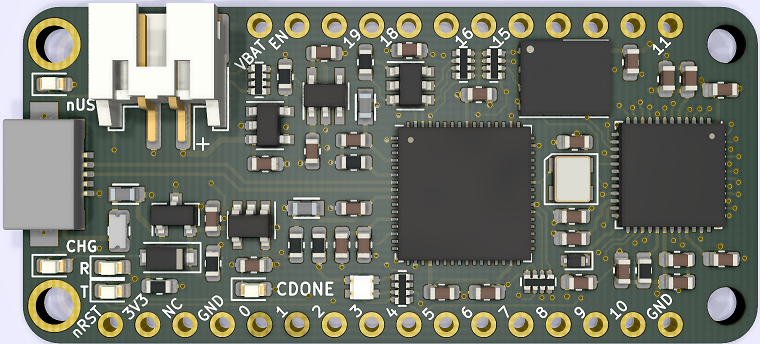
\includegraphics[width=\linewidth]{top_render.PNG}
	\caption{The iCE40-feather FPGA board being utilised.}
\end{centering}
\end{figure}

\begin{figure}[H]
\begin{centering}
	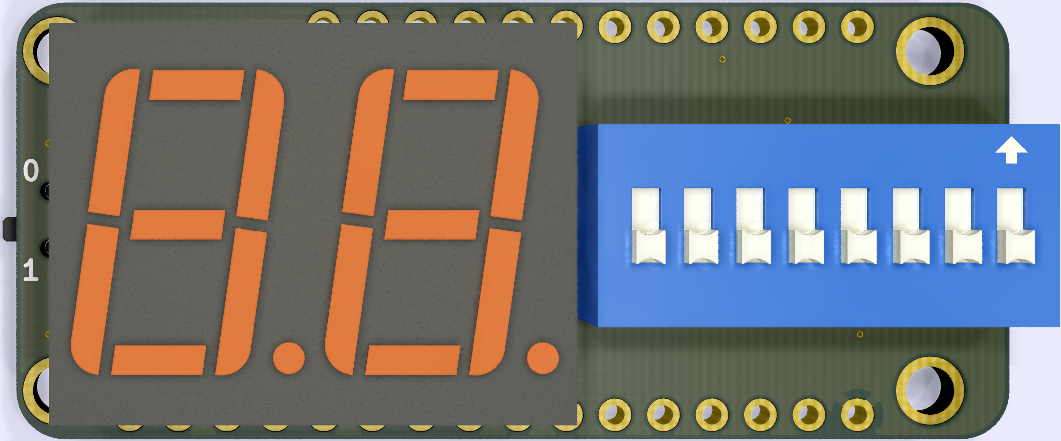
\includegraphics[width=\linewidth]{7segment_render.PNG}
	\caption{The seven segment and DIP switch FeatherWing.}
\end{centering}
\end{figure}
\newpage
\section{Getting to Blinky}
Due to time constraints, it is suggested that you install the toolchain and get a blinking LED on your iCE40-feather before attending the workshop. If you have not already installed the required Yosys, NextPNR, and IceStorm tools, follow the instructions in \texttt{install.md}. If you do not have the FPGA dev board, read the instructions in \texttt{README.md} and get in contact with Josh. \\

\noindent
With the toolchain installed and hardware in hand, it is now time to blink some LEDs! If you have not already done so, clone the repository and open the blink directory.\\

\noindent
\textbf{git clone https://github.com/joshajohnson/WTFpga} \\
\textbf{cd WTFpga/blink}\\

\noindent
Now its time to walk through the process of synthesizing an FPGA design of your own and uploading it to the FPGA. We will be using the amazing open source tools called IceStorm, NextPNR and Yosys. 
\begin{itemize}
		\item Ensure that the FPGA is connected via a USB cable to your computer. 
		\item Open the command line in the \texttt{WTFpga/blink} folder.
		\item Build and upload the gateware by typing \textbf{make prog} into the terminal. 
			\begin{itemize}
				\item NOTE: Windows users may need to run \textbf{make prog} twice due to path issues with the iceprog execuitable. 
			\end{itemize}
		\item Ensure that the led marked nUSR is blinking. If not it's time to begin troubleshooting!
			\begin{itemize}
				\item NOTE: Windows users may need to update drivers used with the FTDI IC used for USB to Serial communications. Check the install notes in \texttt{install.md}.
			\end{itemize}
		\item Once you get the LED blinking, open the file \texttt{blink.v} and have a look around. See if you can change the frequency of the blinking LED by altering the code. 
		\item After changing \texttt{blink.v} and saving it, run \textbf{make prog} again and confirm the frequency changes. 
\end{itemize}
If you have made it this far, congratulations! You have successfully programmed your FPGA, and can now attend the WTFpga workshop knowing that you'll hit the ground running. If you are having issues programming the board, get in contact with Josh and he will lend a hand troubleshooting. 
\newpage
\section{Reading Verilog}
Now that we know how to use the tools to configure our FPGA, let’s start by examining some simple Verilog code. Programming languages give you different ways of storing and passing data between blocks of code. Hardware Description Languages (HDLs) allow you to write code that defines how things are connected. 

\begin{itemize}
	\item \textbf{cd} to the directory\textbf{wtfpga-lab} and open wtfpga.v in the text editor of your choosing.
	\item Our module definition comes first, and defines all the inputs and outputs to our system. Can you locate them on your board?
	\item Next are wire definitions. Wires are used to	directly connect inputs to one or more outputs.
	\item Next are parallel assign statements, all of these assignments are always happending, concurrently. 
	\item Next are always blocks. These are blocks of statements that happen sequentially, and are triggered by the sensitivity list contained in the following @().
	\item Finally we can instantiate modules. There are a few already instantiated but not really used for anything yet.
\end{itemize}
\noindent
Now let’s try and map our board’s functionality to the Verilog that makes it happen.
\begin{itemize}
	\item What happened when you moved the DIP switches?
	\item Can you find the DIP switches in the module definition? What are they named?
	\item Can you find the assignments which use each of the switches? What are the assigned to?
	\item Can you follow the assignments to an output?
	\item Do you notice anything interesting about the order of the assign statements?
\end{itemize}
\noindent
You should be able to trace the DIP switches inputs, through a number of wires, to seven segment outputs. You should also note that the seven segment display is inverted, the reasoning of which will be explained later. 

Note that these aren't sequential commands. All of these things happen at once. It dosen't actually matter what order the assgn statements occur. 
\newpage
\section{Making Assignments}
Let’s start with some minor changes to our Verilog, then configure our board. First, we will make modifications to the file. 
\begin{itemize}
	\item Remove all of the \texttt{seg[x] = sw[x]} assignments from the file 
	\item Replace the previous assignments with \texttt{assign seg[6:0] = $\sim$sw[6:0]}
\end{itemize}
\noindent
Next, we need to create a new configuration for our FPGA. Brace yourself - it will be really quick! ;-)
\begin{itemize}
	\item In the command line terminal that we opened earlier, type \textbf{make prog}, and press enter. Windows users, remember you may have to run \textbf{make prog} twice due to the joys of iceProg. 
\end{itemize}
\noindent
You should see some text scroll by and the new design should be uploaded and running within a few seconds. If we were using proprietary tools (Vivado or Quartus) as we did in V1 and V2 of this workshop the synthesis would take approximately 8 minutes depending on the computer used. We used these 8 minutes to talk about the synthesis process itself. Even though we don’t have to wait that long, let’s talk what the software is doing and what tools are used to accomplish those steps. It is bit different from a software compiler.

\begin{itemize}
	\item First, the software will synthesize the design - turn the Verilog code into basic logical blocks, optimizing it in the process using yosys. (http://www.clifford.at/yosys/)
	\item Next, the tools will implement the design. This takes the optimized list of registers and assignments, and places them into the logical blocks available on the specific FPGA we have configured, then routes the connections between them using the tool called nextpnr. (https://github.com/YosysHQ/nextpnr)
	\item When that completes, the fully laid out 	implementation needs to be packaged into a 	format for programming the FPGA. There are a 	number of options, but we will use a .bit bitstream file for programming over SPI using icePack from the IceStorm tool collection.
	(http://www.clifford.at/icestorm/)
	\item Hopefully everything will go as planned. If you have issues, look in the console for possible build errors. If you have trouble, ask for help!
	\item Finally, the .bin file needs to be sent to the FPGA over USB. When this happens, the demo configuration will be cleared and the new design will take its place using the iceprog tool.
\end{itemize}
\noindent
Check what happens when you move the DIP switches. Does it function as you expect? What has changed from last time?

\newpage
\section{Combinational Logic}
Simple assignments demonstrate the parallel nature of FPGAs, but combinational logic makes it much more useful. We’re going to write a small module (like a procedure) that will convert the binary value shown on the DIP switches into a hex digit on the 7-segment display.

\begin{figure}[H]
	\begin{centering}
		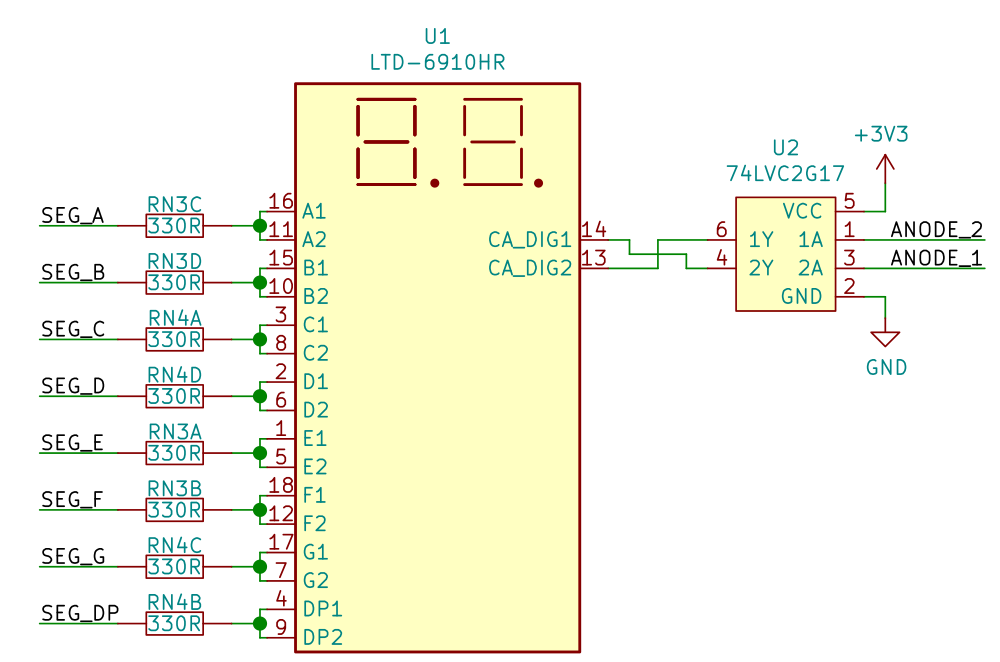
\includegraphics[width=\linewidth]{sevenSeg.png}
		\caption{Schematic for the seven segment display.}
	\end{centering}
\end{figure}
\noindent
There are 7 \texttt{seg[]} output wires that control which LEDs are on or off, and correspond from \texttt{A} to \texttt{G} on the display. There are two anode wires connected through buffers to select which digit is on, and corresponds to \texttt{CA\_DIG1} and \texttt{CA\_DIG2} on the right. To display two different characters, we need to cycle between them fast enough so that they persist in the eye. All of the code to generate the clock (clockDiv.v) and multiplex the display (dispMux.v) is already written and included in the project, giving direct access to each of the displays as disp0 and disp1.
\end{document}